\documentclass[a4paper,12pt]{report}
\usepackage[spanish, es-tabla]{babel}
\usepackage[utf8]{inputenc} 
\usepackage[margin=1in]{geometry}%margenes
\usepackage{graphicx}
\usepackage{setspace}
\onehalfspace %para espacio y medio
\setlength\parindent{0pt}%elimina sangria
\pagenumbering{gobble}%elimina nro de pag
\usepackage{natbib}%para reducir espacio entre items de la biblo

\begin{document}

{\Large \textbf{Título:}} “Análisis de Identificadores para Abstraer conceptos del Dominio del \mbox{Problema”}
\vskip0.5cm
{\Large \textbf{Autor:}} Javier Azcurra Marilungo.
\vskip0.5cm
{\Large \textbf{Dirección:}}
\begin{itemize}
%\itemsep0em%reduce espacio
\item \textbf{Director:} Dr. Mario Marcelo Berón.

\item \textbf{Co-Director:} Dr. Germán Antonio Montejano.
\end{itemize}

{\Large \textbf{Objetivos:}} Los objetivos principales de este Trabajo Final de Licenciatura son:

\begin{itemize}
%\itemsep0em%reduce espacio

\item Extraer identificadores de programas escritos en lenguaje JAVA.

\item Extraer comentarios y literales de programas escritos en lenguaje JAVA.

\item Analizar los identificadores capturados con ayuda de la información extraída en el ítem anterior.

\item Construir en JAVA una herramienta que implemente los ítems anteriores.

\item Evidenciar una aproximación que relacione la salida de un programa con los elementos involucrados que producen dicha salida.

\end{itemize}
{\Large \textbf{Antecedentes}}
\vskip0.5cm
%\hspace{0.5cm}  %Sangria

\hspace{0.5cm} La Ingeniería del Software (IS) es una disciplina encargada de desarrollar sistemas de software de alta calidad. Para conseguir esta meta, la IS abarca, entre otras, tres temáticas importantes: el mantenimiento de software, la evolución de software y la migración de software \cite{RSPMGH02}.

\hspace{0.5cm} El mantenimiento de software \cite{PFT02} es la modificación del sistema después de la entrega al usuario. Esta modificación generalmente se hace para arreglar fallas, mejorar el rendimiento o adaptar el sistema al ambiente cambiante \cite{STD610}. Es por esto, que la comprensión del sistema es crucial para poder mantenerlo correctamente.

\hspace{0.5cm} La evolución de software se encarga de ampliar los sistemas a través del tiempo. Esta ampliación consiste en tomar una versión operativa del software y generar una nueva versión mejorada en su eficiencia \cite{KBVR00}. La comprensión del sistema es necesaria y fundamental antes de comenzar hacia una nueva ampliación.

\hspace{0.5cm} La migración de software es la conversión de un sistema antiguo a un nuevo contexto tecnológico sin alterar la funcionalidad original del mismo. Esta conversión normalmente es costosa y compleja \cite{MMFAF08}. Para reducir estos costos, se aconseja comprender correctamente el viejo sistema.

\hspace{0.5cm} Como se describió en párrafos anteriores, la comprensión de sistemas es fundamental para realizar tareas de mantenimiento, de evolución y de migración de software. Por esta razón, dentro de la IS se encuentra un área conocida como \textit{Comprensión de Programas} (CP). La CP se define como: \textit{una disciplina de la IS encargada de ayudar al
desarrollador a lograr un entendimiento acabado del software, de forma que se pueda analizar disminuyendo el tiempo y los costos}. 

\hspace{0.5cm} El objetivo principal de la CP  \cite{BRM10,MPMR07,MBPHRU10,MAS05} es desarrollar métodos, técnicas y herramientas que faciliten al programador 
el entendimiento de las funcionalidades de los sistemas de software.
Una forma de alcanzar este objetivo consiste en relacionar el \textit{Domino del Problema}, 
es decir la salida del sistema, con el \textit{Dominio del Programa}, o sea 
con las partes del programa utilizadas para generar dicha salida \cite{VMAVA95,MPOB03,BROOK82,AMPM11}.
La construcción de esta relación representa el principal desafío en el contexto de la 
CP. 

\hspace{0.5cm} Una aproximación a la solución del desafío previamente descripto, consiste en armar la siguiente reconstrucción:
I) Elaborar una representación del \textit{Dominio del Problema}. II) Construir una representación para el \textit{Dominio del Programa}. III) Unir las representaciones de los pasos I y II con una \textit{Estrategia de Vinculación}.

\hspace{0.5cm} Para lograr los 3 pasos antedichos, se estudian temáticas importantes asociadas a la CP, algunas de ellas son: los \textit{modelos cognitivos}, la \textit{visualización de software}, la \textit{interconexión de dominios}, la \textit{administración de la información}, la \textit{extracción de la información}. 

\hspace{0.5cm} Este trabajo final está orientado al estudio técnicas de \textit{extracción de información}, por ende, se hará más hincapié en ese tema. Sin embargo, el resto de las temáticas no dejan de ser importantes y constituyen amplias iniciativas de investigación en el área de la CP.

\hspace{0.5cm} La \textit{extracción de la información consiste en el uso/desarrollo de técnicas que permiten extraer información desde el sistema de estudio}. Dependiendo de las necesidades del Ingeniero del Software, la información extraída puede ser estática o dinámica.
 
\hspace{0.5cm}La información dinámica se extrae del sistema en tiempo de ejecución \cite{THBE99, TERD01}. Las técnicas encargadas de extraer este tipo de información, insertan sentencias nuevas en el código fuente del programa. La finalidad de las nuevas sentencias es registrar las actividades realizadas durante la ejecución del programa. Esta inserción de sentencias nuevas no deben alterar la funcionalidad original del programa.
%\hspace{0.5cm}Las sentencias nuevas insertadas pueden simplemente imprimir las secciones que se están ejecutando. Más complejo aún, se pueden agregar un conjunto de sentencias nuevas que reemplacen a otro conjunto (sin alterar la funcionalidad original) para hacer un estudio más preciso en ciertas partes del código.
%El volumen de información extraída puede ser de gran magnitud. Es por esto, que el encargado de hacer el análisis dinámico debe conocer con claridad los lugares estratégicos donde colocar las sentencias.

%\hspace{0.5cm}La instrumentación de código es una de las técnicas más conocidas del análisis dinámico \cite{THBE99}. Esta técnica, inserta sentencias para crear trazas de ejecución en distintas partes del código. Las trazas clarifican la ejecución del programa mejorando la comprensión del mismo.

%\hspace{0.5cm}El análisis estático es tan importante como el análisis dinámico.

\hspace{0.5cm}Por otro lado, la extracción de información estática a diferencia de la dinámica, no requiere ejecutar el sistema. Para extraer información estáticamente se utilizan técnicas de compilación tradicionales, estas técnicas realizan un análisis sintáctico y semántico en el código fuente del sistema de estudio \cite{TERD01, AHUL06}. Durante este análisis se capturan elementos estáticos que están presentes en el código.


%\hspace{0.5cm}Para llevar a cabo estos análisis se recorre el árbol de sintaxis abstracta (ASA) \cite{AHUL06}. En la fase de compilación, el ASA se construye a medida que se analiza el código.

%\hspace{0.5cm}Una forma de construir el ASA es por comprensión \cite{AHUL06}, esta forma se logra en la etapa del análisis sintáctico durante el proceso de compilación del código. Es la más sencilla y se utiliza en tareas de chequeos de tipos, generación de código, construcción de grafo de funciones, entre otras.

%\hspace{0.5cm}Otra forma de elaborar el ASA es por extensión \cite{AHUL06}, esta forma se usa para hacer análisis más complejos en el código. También extrae mayor cantidad de información en tiempo de compilación. Algunos ejemplos de tareas que se pueden realizar son, extracción de identificadores, extracción de funciones y tipos y demás objetos presentes en el código. 

%\hspace{0.5cm}El ASA por extensión también se usa para resolver conflictos a nivel semántico, como es el caso de borrar referencias a variables redundantes, detectar funciones o estructuras a través del uso de punteros.

\hspace{0.5cm} El correspondiente trabajo final hará más énfasis en la extracción de información estática. Cabe destacar que la dinámica también es importante, sin embargo su análisis requiere de otro tipo de aproximaciones que escapan a los objetivos de este trabajo. 

\hspace{0.5cm}Como bien se explico en párrafos precedentes, se pueden extraer distintos objetos del código fuente de forma estática usando técnicas de compilación, y sin la necesidad de ejecutar el código. 

%=======================================

\hspace{0.5cm}Un elemento estático que abunda en los códigos son los identificadores. Estudios realizados sobre 2.7 millones de líneas de código escritas en JAVA, indican que más del 70\% de los caracteres del código fuente forman parte de un identificador \cite{DFPM05,DMDJ13}.

\hspace{0.5cm} Algunos autores \cite{BCPT99,LFBEX07,EZH08,EHPV09} señalan que los identificadores ocultan información importante del \textit{Dominio del Problema}. Los identificadores de un programa normalmente están compuestos por más de una palabra en forma de abreviatura, por ejemplo: \textsf{inp\_fl\_sys}. Una forma de analizar identificadores y revelar la información oculta que estos contienen, implica realizar los siguientes pasos: I) Extraer los identificadores del código de estudio, II) Aplicar una técnica de división en donde se descompone al identificador en las distintas abreviaturas que lo componen. Por ejemplo: \textsf{inp\_fl\_sys} $\rightarrow$ \textsf{inp fl sys}. III) Por último, emplear una técnica de expansión de abreviaturas que las expande a palabras completas. Por ejemplo: \textsf{inp fl sys} $\rightarrow$ \textsf{input file system}.

\hspace{0.5cm}Para realizar los pasos de división y expansión se recurren a fuentes de palabras/frases dentro del código, tales como: comentarios, literales strings, documentación.
Sin duda, estas son fuentes naturales que ayudan a comprender el código \cite{JDPH08}.
En caso de que estas fuentes sean escasas, una alternativa viable es consultar fuentes de palabras externas al código como es el caso de los diccionarios con palabras en lenguaje natural, entre otros.

\hspace{0.5cm}Por lo antedicho, investigar y construir herramientas que puedan extraer y analizar identificadores desde los códigos JAVA es un aporte al área de CP. En la actualidad existen técnicas que extraen, dividen y expanden identificadores \cite{EZH08, EHPV09, BCPT00, HDD06}. Desafortunadamente, no todas estas estrategias de análisis de identificadores se han programado en herramientas automáticas.
Tomando como iniciativa el problema sobre la falta de herramientas automáticas en el marco de análisis de identificadores, el presente trabajo final de licenciatura pretende aproximar algunas soluciones. 

\hspace{0.5cm} Se construirá una herramienta que extrae los identificadores de programas escritos con lenguaje JAVA. Esta herramienta
también capturará comentarios y literales dentro del código que serán de utilidad a la hora de analizar los identificadores.
Luego la herramienta aplicará técnicas de división y expansión de identificadores que fueron descriptas anteriormente.
%Se va a elaborar un analizador sintáctico en lenguaje JAVA que extrae los identificadores, comentarios y literales encontrados en códigos fuentes escritos en lenguaje JAVA.
%Luego se van a investigar técnicas conocidas de división y de expansión de abreviaturas pertenecientes a identificadores. Finalmente, se procederá a implementar una herramienta que integre algunas técnicas de análisis de identificadores antedichas junto al analizador sintáctico explicado anteriormente. 

\hspace{0.5cm} De esta manera, se obtendrá una herramienta que extrae y analiza información estática contenida detrás de los identificadores.
%\hspace{0.5cm} El correspondiente trabajo final de licenciatura basa su estudio en capturar y abstraer conceptos del dominio del problema a través del análisis de identificadores. Este análisis, será mostrado con la herramienta antedicha, que implementa algunas estrategias conocidas \cite{DFPM05,DMDJ13,EHPV09} de análisis de identificadores en programas JAVA.
Construir una herramienta de estas características es un aporte directo al área de la CP, ya que permite encarar a uno de sus principales desafíos: vincular el \textit{Dominio del Problema} con el \textit{Dominio del Programa}.
\vskip0.5cm

\pagebreak
{\Large \textbf{Metodología}}
\vskip0.5cm

\hspace{0.5cm}La metodología a utilizar en este trabajo final, esta enmarcada por 3 etapas principales:

\begin{itemize}
\renewcommand{\labelitemi}{$\circ$}%icono circulo

\item \textbf{Primera Etapa: Investigación de conceptos orientados a la Comprensión de Programas y a la extracción de información estática.}

\hspace{0.5cm}En esta etapa se incorporan los conocimientos necesarios para llevar adelante este trabajo final. Se investigará sobre comprensión de programas y las áreas que contiene. De todas estas áreas, se hará más hincapié en la extracción de información estática en base al análisis de identificadores presentes en los códigos. Este análisis, servirá para la implementación de técnicas de comprensión de sistemas.

\item \textbf{Segunda Etapa: Elaboración de una estrategia para extraer\\ identificadores.}

%\hspace{0.5cm}Se construirá un analizador sintáctico (parser) encargado de extraer identificadores, comentarios y literales desde los códigos escritos en JAVA. Estos comentarios y literales ayudarán al análisis de identificadores. Para construir este parser, se investigarán herramientas que ayude a la construcción y se elegirá la más adecuada. Se llevarán a cabo las pruebas pertinentes.
\hspace{0.5cm} En esta fase se realiza un estudio de técnicas/herramientas encargadas de la extracción de identificadores, comentarios y literales presentes en códigos de programas escritos en JAVA. Como se describió antes, los comentarios y literales ayudarán a analizar los identificadores. De todas estas técnicas de extracción, se elegirá la más adecuada para ser implementada. Por último, se llevarán a cabo las pruebas pertinentes.



\vskip0.5cm
\item \textbf{Tercera Etapa: Construcción de la herramienta que analiza\\identificadores.}

\hspace{0.5cm}Finalmente, en la última etapa se construye una herramienta que contendrá la estrategia de extracción elaborada en la etapa anterior y también implementa algunas de las técnicas de análisis de identificadores estudiadas en la primer etapa. La finalidad de esta herramienta es extraer y analizar información presente en identificadores ubicados en códigos JAVA. Esta información extraída y analizada, se considera propia del \textit{Dominio del Problema} y es un aporte a la reconstrucción de la relación entre: el \textit{Dominio del Problema} y el \textit{Dominio del Programa}.

\end{itemize}
\pagebreak
{\Large \textbf{\\Plan y cronograma de tareas}}

\begin{enumerate}
\itemsep0em%reduce espacio
\item Estudiar conceptos, técnicas y herramientas sobre la comprensión de programas: con esto se lográ conocer las características relacionadas al ámbito de la comprensión de sistemas.

\item\label{plan1} Investigar conceptos, técnicas y herramientas relacionados al análisis de identificadores: aquí se adquieren los conceptos necesarios para extraer información del \textit{Dominio del Problema}, en base a los identificadores.

%\item Estudiar herramientas automatizadas que generen Analizadores Lexicográficos y Analizadores Sintácticos, se hará preferencia en aquellas que usen gramática de atributos.

\item Investigar técnicas/herramientas que extraigan identificadores, comentarios y literales ubicados en códigos  escritos en lenguaje JAVA.

\item Elaborar un técnica de extracción de identificadores, comentarios y literales elegida en base a la investigación del ítem anterior.

\item Implementar una herramienta en JAVA que  contenga distintas técnicas de análisis de identificadores investigados en el ítem \ref{plan1}. Esta herramienta también contendrá la técnica de extracción elaborada en la etapa anterior.

\item Escribir el informe del trabajo final. Mientras se ejecutan los ítems precedentes, se irá redactando el informe correspondiente al trabajo final.
\end{enumerate}


\begin{figure}[b] %[h] para here [b] para bottom [t] para top
\centerline{%queda centrada mejor la imagen
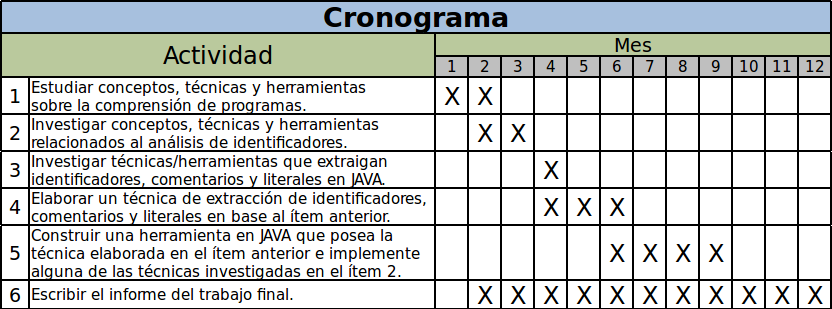
\includegraphics[scale= 0.85]{./crono.png}
}
\end{figure} 

\pagebreak

{\Large \textbf{Recursos}}
\vskip0.5cm
\hspace{0.5cm}El correspondiente trabajo final se llevará a cabo en la Universidad Nacional de San Luis, en el Área Programación y Metodologías de Desarrollo de Software enmarcado en los siguientes proyectos:

\begin{itemize}
\renewcommand{\labelitemi}{$\diamondsuit$}%icono circulo

\item \textit{“Ingeniería del Software: Conceptos Métodos Técnicas y 
Herramientas en un Contexto de Ingeniería de Software en Evolución”} de la Universidad 
Nacional de San Luis. 
Dicho proyecto, es reconocido por el programa de incentivos y es la continuación de 
diferentes proyectos de investigación de gran éxito a nivel nacional e internacional.

\item \textit{“Quixote - Development of Problem Domain Models to Interconnect the Behavioral and Operational Views to Aid in Software Systems Comprehension”} (código de proyecto: PO/09/38).  Quixote es un proyecto bilateral entre la Universidade do Minho (Portugal) y la Universidad Nacional de San Luis (Argentina). Dicho proyecto fue aprobado por el Ministerio de Ciencia, Tecnología e Innovación Productiva de la Nación (MinCyT)\footnote[1]{www.mincyt.gov.ar/}, y la Fundação para a Ciência e Tecnología (FCT)\footnote[2]{www.fct.mctes.pt/} de Portugal. 

\end{itemize}

\hspace{0.5cm}Ambos entes soportan económicamente la realización de diferentes misiones de investigación desde Argentina a Portugal y viceversa, como así también la presentación y publicación de artículos en diferentes congresos nacionales e internacionales.\\

\hspace{0.5cm}Por otro lado, el equipamiento necesario es una PC con el sistema Linux, impresora y papel para realizar las impresiones del informe. También se hará uso de internet, de material bibliográfico provisto por la biblioteca “Antonio Esteban Agüero”; y  de material provisto por las librerías digitales a las que se tiene acceso desde la Universidad Nacional de San Luis.


%========================================

\renewcommand{\bibname}{\vspace{-3cm} \Large \textbf{Bibliografía}}
\setlength{\bibsep}{1.5pt}
\bibliographystyle{plain}%{alpha}
\bibliography{biblo}
\nocite{*}%para que imprima toda la referencias sin necesidad de citar

{\Large \textbf{\\Firma de alumno y asesores}}

\end{document}